\documentclass[a4paper, 10pt, final, garamond]{book}
\usepackage{cours-preambule}
\graphicspath{{./figures/}}
\addto\captionsfrench{\renewcommand{\figurename}{Fig.}}

\makeatletter
\renewcommand{\@chapapp}{Contr\^ole de connaissances}
\makeatother

% \toggletrue{student}
% \toggletrue{corrige}
\renewcommand{\mycol}{black}
% \renewcommand{\mycol}{gray}

\begin{document}
\setcounter{chapter}{2}

\settype{enon}
\settype{solu}

\chapter{Électrocinétique~: ARQS et résistances}

\begin{enumerate}[label=\sqenumi, leftmargin=10pt]
	\item[n]{4} %
	Démontrer la relation de conjugaison de \textsc{Newton}. Un schéma
	est attendu.
	\smallbreak
	\begin{isd}[righthand ratio=.3]
		\psw{%
			On utilise le théorème de \textsc{Thalès} dans les triangles F$'$OH et
			F$'$A$'$B$'$, en remarquant que $\obarr{OH} = \AB$, et les
			triangles FAB et FOH' pour avoir
			\begin{gather*}
				\frac{\obarr{A'B'}}{\obarr{OH}} = \frac{\ABp}{\AB} \stm{=}
				\frac{\obarr{F'A'}}{\obarr{F'O}}
				\qqet
				\frac{\obarr{OH'}}{\obarr{AB}} = \frac{\ABp}{\AB} \stm{=}
				\frac{\obarr{FO}}{\obarr{FA}}
				\\\Lra
				\boxed{\OFp\times\OF = \obarr{F'A'}\obarr{FA}}
				\hspace{12pt}
				\pt{1}
			\end{gather*}
		}%
		\vspace{-10pt}
		\tcblower
		\begin{center}
			\sswitch{%
				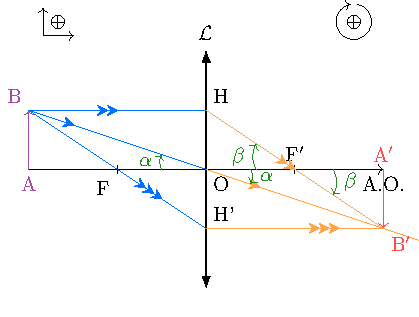
\includegraphics[width=.8\linewidth, draft=true]{lent_conv-demo}
			}{%
				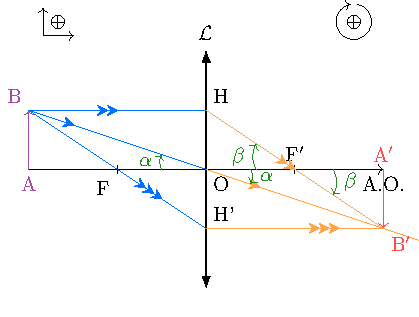
\includegraphics[width=.8\linewidth]{lent_conv-demo}
			}%
      \vspace{-15pt}
			\captionof{figure}{Schéma \protect \pt{1}}
			\label{fig:lent_rc}
		\end{center}
			\vspace{-30pt}
	\end{isd}
	\item[n]{2} %
	Établir les liens entre les courants et tensions en \textbf{nommant les
		nœuds et les mailles sur le schéma}.
	\smallbreak
	% \vspace{-30pt}
	\begin{isd}[interior hidden, lefthand ratio=.4]
		\vspace{-15pt}
		\begin{center}
			\sswitch{%
				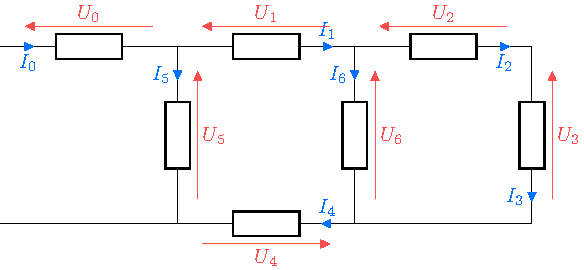
\includegraphics[width=\linewidth]{exer_ldnm_plain}
			}{%
				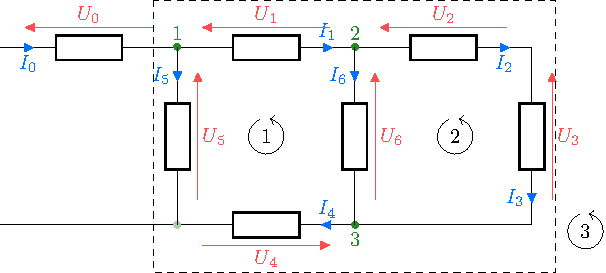
\includegraphics[width=\linewidth]{exer_ldnm}
			}%
			% \vspace{-15pt}
			% \captionof{figure}{Schéma \protect\pt{1}}
		\end{center}
		\vspace{-30pt}
		\tcblower
		\begin{isd}[sidebyside align=top]
			\vspace{-15pt}
			\tcbsubtitle{\fatbox{Lois des nœuds} \pt{1}}
      \vspace{-15pt}
			\psw{%
				\begin{itemize}
					\item $I_2 = I_3$ par unicité à droite~;
					\item $I_0 = I_1 + I_5$ par LdN 1~;
					\item $I_1 = I_2 + I_6$ par LdN 2~;
					\item $I_3 + I_6 = I_4$ par LdN 3.
				\end{itemize}
			}%
			\vspace{-15pt}
			\tcblower
			\vspace{-15pt}
			\tcbsubtitle{\fatbox{Lois des mailles} \pt{1}}
      \vspace{-15pt}
			\psw{%
				\begin{itemize}
					\item $U_4 + U_6 + U_1 = U_5$ par LdM 1 ;
					\item $U_3 + U_2 = U_6$ par LdM 2 ;
				\end{itemize}
			}%
			\vspace{-15pt}
		\end{isd}
	\end{isd}
	\item[n]{5} %
	Représenter et flécher deux résistances $R_1$ et $R_2$ en série,
	puis démontrer l'expression de la résistance équivalente $R_{\rm eq}$.
	\smallbreak
	\begin{isd}[lefthand ratio=.3]
		\vspace{-15pt}
		\begin{center}
			\sswitch{%
				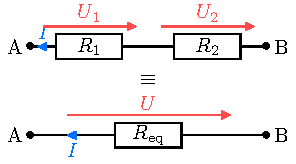
\includegraphics[width=\linewidth, draft=true]{rserie}
			}{%
				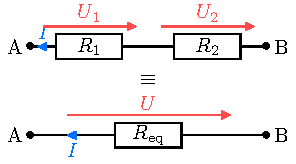
\includegraphics[width=\linewidth]{rserie}
			}%
			\vspace{-15pt}
			\captionof{figure}{$R$ série \protect\pt{1}\psw{+}\protect\pt{1}}
		\end{center}
		\vspace{-15pt}
		\tcblower
		\vspace{-15pt}
		\psw{%
			\begin{align*}
				U                 & \stm{=} U_1 + U_2
				\\\Lra
				U                 & \stm{=} R_1I + R_2I
				\\\Lra
				U                 & = (R_1 + R_2)I
				\\\Lra
				\Aboxed{R\ind{eq} & \stm{=} R_1 + R_2}
				\qed
			\end{align*}
		}%
		\vspace{-15pt}
	\end{isd}
	\item[n]{5} %
	Représenter et flécher deux résistances $R_1$ et $R_2$ en parallèle, puis
	démontrer l'expression de $R_{\rm eq}$.
	\smallbreak
	\begin{isd}[lefthand ratio=.3]
		\vspace{-15pt}
		\begin{center}
			\sswitch{%
				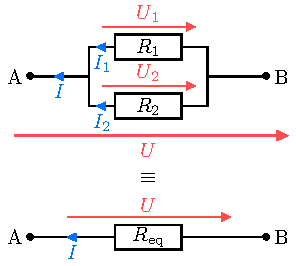
\includegraphics[width=.7\linewidth, draft=true]{rpara}
			}{%
				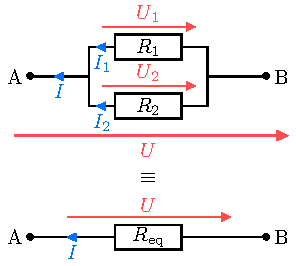
\includegraphics[width=.7\linewidth]{rpara}
			}%
			% \vspace{-15pt}
			\captionof{figure}{$R$ parallèle \protect\pt{1}\psw{+}\protect\pt{1}}
		\end{center}
		\vspace{-15pt}
		\tcblower
		\vspace{-15pt}
		\psw{%
			\begin{align*}
				I                   & \stm{=}
				I_1 + I_2 =
				\left( \frac{1}{R_1} + \frac{1}{R_2} \right)U
				\\\Lra
				\frac{1}{R\ind{eq}} & \stm{=}
				\left( \frac{1}{R_1} + \frac{1}{R_2} \right)
				\\\Lra
				\Aboxed{R_{\rm eq}  & \stm{=}
					\frac{R_1R_2}{R_1+R_2}}
			\end{align*}
		}%
		\vspace{-15pt}
	\end{isd}
	\item[n]{4} %
	Représenter un pont diviseur de tension avec 2 résistances et démontrer la
	relation associée pour $k$ résistances.
	\smallbreak
	\begin{isd}[lefthand ratio=.30]
		\vspace{-15pt}
		\begin{center}
			\sswitch{%
				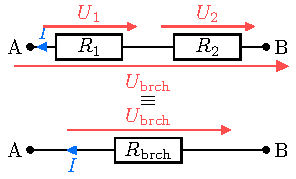
\includegraphics[width=\linewidth, draft=true]{rserie_divtens}
			}{%
				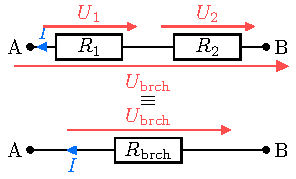
\includegraphics[width=\linewidth]{rserie_divtens}
			}%
			\vspace{-15pt}
			\captionof{figure}{PdT \protect\pt{1}\psw{+}\protect\pt{1}}
		\end{center}
		\tcblower
		\psw{%
			On part de ce qui est partagé dans le circuit, ici l'intensité~:
			\begin{gather*}
				I = \frac{U\ind{brch}}{R\ind{brch}}
				\stm{\qet}
				I = \frac{U_k}{R_k}
				\qqso
				\boxed{U_k \stm{=} \frac{R_k}{R\ind{brch}U\ind{brch}}}
				\qed
			\end{gather*}
		}%
		\vspace{-15pt}
	\end{isd}
  \item[n]{+2} %
    Explain the law of reflection using wavelight formalism.
    \smallbreak
    \psw{%
      The lightwaves hitting silver atoms make them vibrate and emit spherical
      waves. These waves cancel out in all directions but the reflected one.
    }%
\end{enumerate}
\vspace{-30pt}

\ifstudent{%
	\begin{tikzpicture}[remember picture, overlay]
		\node[anchor=north west, align=left]
		at ([shift={(1.4cm,0)}]current page.north west)
		{\\[5pt]\Large\bfseries Nom~:\\[10pt]\Large\bfseries Prénom~:};
		\node[anchor=north east, align=right]
		at ([shift={(-1.5cm,-17pt)}]current page.north east)
		{\Large\bfseries Note~:\hspace{1cm}/20};
	\end{tikzpicture}
}%
\end{document}
